\chapter{Fundamentos e Revisão de Literatura}
\label{chap:fundamentacao}
É necessário definir alguns termos, técnicas e/ou ferramentas para o entendimento deste trabalho. Por exemplo, a conceituação formal de sensibilidade ao contexto é muito importante, uma vez que constitue-se da técnica de obtenção dos dados. Como complemento à sensibilidade ao contexto define-se o que é o ZooKeeper, a ferramenta utilizada para transmissão dos dados coletados. Além disso, é relevante que exista a compreensão de como o Apache Hadoop, seu escalonamento e o paradigma de programação utilizado funcionam, bem como quais trabalhos já foram feitos neste âmbito.

%-------------------------------------------------------------------

\section{Sensibilidade ao Contexto}
\label{sec:ctx}
Quando um usuário acessa um site por meio de um dispositivo móvel este site carrega automaticamente sua versão \emph{mobile}, a qual possui alterações que aumentam a compatibilidade com o tipo de dispositivo sendo utilizado. Uma situação semelhante ocorre quando navegadores utilizam dados de localidade para melhorar os resultados de um motor de buscas, mostrando primeiro os resultados mais relacionados com a região ou idioma do usuário. Nota-se que nas duas situações a aplicação utiliza dados específicos, o tipo do dispositivo e a localização do usuário, coletados no momento da execução e utiliza-os para adaptar o seu funcionamento de maneira a oferecer maior conforto ou usabilidade ao usuário. Estes dados representam o contexto dos usuários, o qual é definido por \cite{Dey} como qualquer informação que pode ser utilizada para caracterizar a situação de uma entidade (pessoa, lugar ou objeto) considerada relevante para a interação entre usuário e aplicação.

Sendo assim, se uma aplicação é capaz de coletar informações sobre a situação do sistema no qual está sendo executada, ela é capaz de coletar informações de contexto. Porém a simples coleta não aumenta, de fato, o desempenho desta aplicação, é necessário que ela seja capaz de responder às mudanças do ambiente detectadas. Esta capacidade de detecção e reação é caracterizada como sensibilidade ao contexto por \cite{Maamar} e vai ao encontro da definição de \cite{Baldauf} em que o sistema deve detectar mudanças e adaptar suas operações sem intervenção explícita do usuário, aumentando assim a usabilidade e eficácia da aplicação.


%-------------------------------------------------------------------

\section{Hadoop}
O \textit{framework} Apache Hadoop origina-se de outro projeto da Apache, o Apache Nutch \cite{Nutch}. O Apache Nutch iniciou em 2002 como um motor de buscas de código livre, porém o projeto encontrou problemas devido a sua arquitetura. Quando a Google publicou um artigo em 2003 descrevendo a arquitetura utilizada no seu sistema de arquivos distribuídos, chamado GFS (\textit{Google File System}), os desenvolvedores do Nutch notaram que uma arquitetura semelhante resolveria seus problemas de escalabilidade. A implementação da ideia foi iniciada em 2004 e o resultado foi nomeado \textit{Nutch Distributed Filesystem} (NDFS). Contudo, a medida em que o projeto se desenvolvia o propósito original do Nutch era deixado em segundo plano, o que culminou na criação de um novo projeto em 2006. Este novo projeto foi nomeado Apache Hadoop e possui o propósito de facilitar o processamento distribuído através do paradigma MapReduce.

\subsection{Arquitetura geral do \emph{Apache Hadoop}}
O \textit{framework} Apache Hadoop é organizado em uma arquitetura de mestre-escravo e possui dois serviços principais, o serviço de armazenamento (HDFS - Hadoop Distributed File System) e o de processamento (YARN - Yet Another Resource Negotiator), os quais podem ser vistos na Figura \ref{fig:ArquiteturaHadoop}.

\begin{figure}[!ht]
\centering
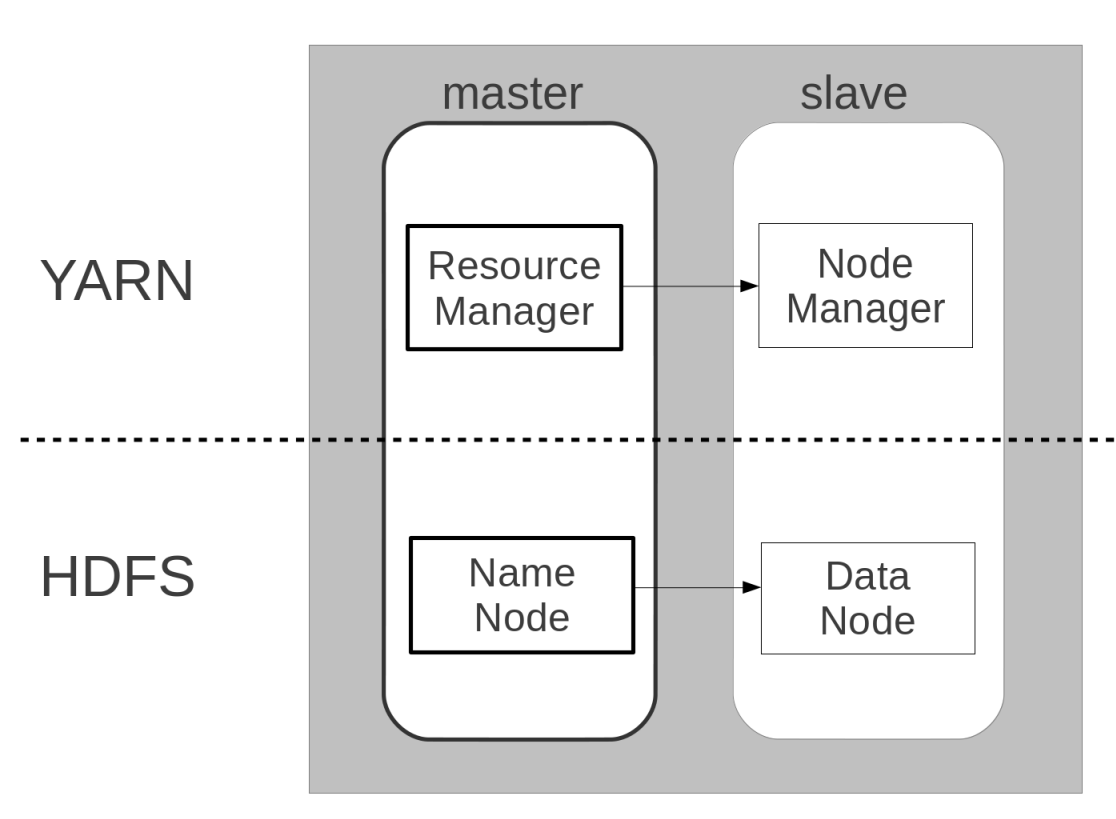
\includegraphics[width=0.7\textwidth]{figuras/Figura08-HadoooArchGeral.png}
\caption{Arquitetura geral do Apache Hadoop}
\label{fig:ArquiteturaHadoop}
\end{figure}

Nesta figura, é possível notar a existência de 4 componentes do \textit{framework}. Os componentes acima da linha pontilhada pertencem ao YARN, sendo o Resource Manager e o Node Manager os serviços mestre e escravo respectivamente. O HDFS é composto pelos componentes abaixo da linha pontilhada, sendo o Name Node e o Data Node os serviços mestre e escravo respectivamente.

\subsubsection{HDFS}
Grande parte do ganho de desempenho oferecido pelo Hadoop decorre do comportamento de levar o processamento até os dados, ou seja, todo processamento é feito com dados locais. Esta abordagem só é possível de ser realizada graças ao HDFS. Dentro do Name Node são mantidas informações de quais partes de quais arquivos estão em cada Data Node, ou seja, todos os arquivos estão divididos num grande HD distribuído e o mestre sabe exatamente quais blocos cada escravo possui. Dessa forma cada nó executa tantos Maps ou Reduces quanto a quantidade de arquivos locais permitir, diminuindo a necessidade de utilizar a rede para transferência de arquivos e deixando-a disponível para ser utilizada para a transferência dos resultados que são os dados já reduzidos. Um problema dessa abordagem é que o Hadoop possui uma latência muito alta, sendo desaconselhável o uso do Hadoop em aplicações críticas ou de tempo real \cite{BookHadoop}. A Figura \ref{fig:ArqHDFS} apresenta um esquema básico da arquitetura do HDFS.

\begin{figure}[!hbtn]
   \centering
   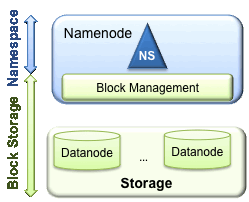
\includegraphics[width=8cm]{figuras/Figura07-HDFS.png}
   \caption{Arquitetura geral do HDFS \cite{HDFS}}
   \label{fig:ArqHDFS}
\end{figure}

\subsubsection{YARN}
Sendo o componente do Apache Hadoop responsável pela execução do \emph{MapReduce}, o YARN realiza tarefas de gerenciamento e execução do processamento. Um dos objetivos do YARN é tornar a tarefa de processamento totalmente independente das tarefas de armazenamento, possibilitando que o \textit{cluster} seja utilizado em conjunto com outras ferramentas que não utilizem o paradigma MapReduce \cite{Vavilapalli}. A Figura \ref{fig:ArqYARN} apresenta um esquema básico da arquitetura do YARN.

\begin{figure}[!hbtn]
   \centering
   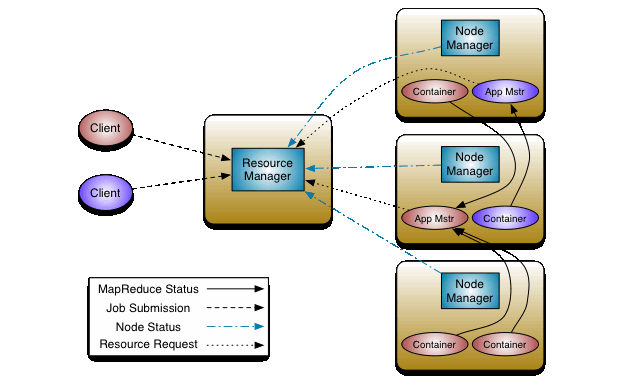
\includegraphics[width=12cm]{figuras/Figura06-YarnArch.png}
   \caption{Arquitetura geral do YARN \cite{YARN}}
   \label{fig:ArqYARN}
\end{figure}

Na imagem é possível observar dois novos componentes do YARN. O primeiro é um componente do Node Manager, possuindo o papel de um escalonador interno de cada aplicação (Application Master - referenciado na imagem como App Mstr), sendo também conhecido por escalonador de tarefas. Considera-se que tarefas sejam uma fração do processamento das aplicações, ou seja, cada tarefa de Map ou Reduce corresponde a uma das divisões que serão processadas em paralelo. É importante não confundir este componente com o escalonador de aplicações, o qual é um componente do Resource Manager e pode ser melhor compreendido com a leitura da Seção \ref{sec:HadSched}. O outro componente presente na figura é o Container, o qual representa uma alocação de recursos em um nó qualquer do \textit{cluster}. A importância do container vem do fato de que todas as tarefas são executadas em uma instância de container.

É importante notar que existem 2 instâncias de Application Master na figura e que elas estão, assim como os clientes e os containers, coloridas de rosa ou roxo para indicar que pertencem à mesma aplicação, ou seja, o cliente rosa lançou uma aplicação que possui o Application Master e mais 3 containers de processamento. Nota-se também que o Resource Manager recebe informações tanto dos clientes quanto dos Node Managers e Application Masters, centralizando todas elas para um controle dos recursos disponíveis.

\subsection{Configuração do ambiente de execução do Hadoops}
Uma característica importante do Hadoop tem relação com sua configuração. Sabe-se que todo sistema necessita de uma configuração por parte de seu administrador, e o Hadoop não é diferente com relação a isso. O Hadoop utiliza uma série de arquivos em cada um dos nós do \textit{cluster} para definir sua configuração. Estes arquivos de configuração são, na verdade, arquivos XML compostos por parâmetros de configuração e valores que influenciam o comportamento do \textit{framework} no \textit{cluster}. Para conhecimento, esses arquivos são: \textit{core-site.xml, yarn-site.xml, mapred-site.xml} e \textit{hdfs-site.xml}. Cada um destes arquivos possui propriedades de um serviço do Hadoop, como exemplo o arquivo \textit{hdfs-site.xml} é responsável pela configuração do HDFS na máquina em questão. 

É importante salientar que para a execução distribuída, ao menos algumas propriedades mais simples dos arquivos de cada nó, seja este mestre ou escravo, devem ser configuradas. No caso do administrador desejar fazer uma configuração mais específica de cada nó escravo ele deverá editar as propriedades nos arquivos de cada um dos nós. Caso o administrador não queira configurar os nós escravos, eles irão executar com base nos valores \textit{default}, contudo esta decisão irá, provavelmente, afetar o desempenho do \textit{cluster} devido à má configuração.

\section{MapReduce}
O paradigma de programação MapReduce é, geralmente, associado com implementações que processam e geram grandes conjuntos de dados. Neste paradigma, todo processamento é dividido em duas etapas, a etapa de Map e a de Reduce, originárias das linguagens funcionais. Como consequência da divisão em duas etapas, o resultado da primeira é a entrada da segunda e esta transferência de dados é baseada em de pares de chave e valor, o que torna possível expressar uma vasta gama de tarefas reais por meio deste paradigma \cite{Dean}.

O \textit{work-flow} padrão de uma aplicação MapReduce inicia com a entrada de dados, que será dividida em \textit{n} partes e cada parte será processada individualmente por uma tarefa Map. O resultado das tarefas Map já será na forma de pares chave e valor, que serão passados como entrada para as tarefas de Reduce. Por sua vez, as tarefas de Reduce irão receber todos os pares com determinada chave e aplicar um algoritmo sobre os pares, fornecendo uma saída inteligível \cite{BookHadoop}.

%TODO citação
A naturalidade do paralelismo deste paradigma, torna a programação da aplicação mais simples. Ao utilizar o paradigma do MapReduce o programador deve apenas pensar em uma solução que siga o \textit{work-flow} do paradigma, e o parelelismo será inerente.

\section{ZooKeeper}
O ZooKeeper é um projeto da Apache e fornece ferramentas eficientes, confiáveis e tolerantes à falha para a coordenação de sistemas distribuídos \cite{Hunt2010}. Inicialmente, o ZooKeeper foi implementado como um componente do Hadoop e virou um projeto próprio conforme cresciam suas funcionalidades e sua utilização em outras aplicações. 

No caso deste trabalho, os serviços do ZooKeeper são utilizados para monitorar e transmitir as informações de contexto coletadas nos nós escravos. No ZooKeeper existe um componente chamado \textit{znode} onde é possível inserir qualquer tipo de dado e todos as instâncias de clientes e servidores (no caso de um servidor replicado) possuem acesso à este \textit{znode}. A comunicação é feita através de processos que atualizam e processos que lêem o conteúdo destes componentes.


%-------------------------------------------------------------------

\section{Escalonadores para o Hadoop}
\label{sec:HadSched}
Apesar de existirem dois níveis de escalonamento no Hadoop, escalonamento de aplicações e de tarefas, este trabalho influencia apenas o escalonamento de aplicações. O escalonador de aplicações gerencia qual será a primeira aplicação a receber um container para seu escalonador de tarefas e quais serão os escalonadores de tarefa que receberão recursos para execução \cite{BookHadoop}. O Hadoop já inclui alguns escalonadores que oferecem maneiras diferentes para a realização do escalonamento de aplicações. Para alterar o escalonador utilizado é necessário alterar uma propriedade no arquivo \textit{yarn-site.XML} e reiniciar o Resource Manager.

Dentre os escalonadores incluídos no Hadoop, o mais simples é o Hadoop Internal Scheduler que utiliza o algoritmo FIFO e tem boa performance em \textit{clusters} onde não existe competição por recursos. Este escalonador suporta até 5 níveis de prioridade, porém a decisão da próxima aplicação a ser executada sempre levará em consideração a hora de submissão.

Um pouco mais complexo que o Internal Scheduler, o Fair Scheduler é utilizado principalmente para o processamento de lotes de aplicações pequenas e rápidas, opera baseado em um escalonamento de dois níveis e possui o objetivo de realizar uma divisão justa dos recursos. O primeiro nível realiza o escalonamento na forma de filas para cada usuário ativo, dividindo os recursos do cluster igualitariamente entre as filas. Enquanto isso, o segundo nível realiza o escalonamento dentro de cada fila da mesma forma que o Internal Scheduler \cite{FairScheduler}. 

A terceira opção, e também o padrão do Hadoop nas últimas versões, é o Capacity Scheduler, o qual foi projetado para a utilização compartilhada do Hadoop e busca a maximização do \textit{throughput} e da utilização do \textit{cluster}. Seu funcionamento baseia-se em garantias mínimas de capacidade para os usuários, ou seja, qualquer usuário terá sempre uma garantia mínima de recursos para utilização. Porém quando algum usuário está com seus recursos ociosos o escalonador repassa a capacidade deste usuário  para aqueles que estão utilizando o \textit{cluster}. Esta estratégia fornece elasticidade com um bom custo benefício, uma vez que diferentes organizações possuem diferentes horários de pico para o processamento de informações. Este escalonador é capaz de rastrear os recursos registrados no Resource Manager, embora esta informação pode não ser consistente com a realidade, e monitorar quais deles estão livres e quais estão sendo utilizados pelo \textit{framework} \cite{CapacityScheduler}.

A existência destes escalonadores adiciona flexibilidade no gerenciamento do \textit{framework}. Apesar disso, os escalonadores disponíveis não detectam nem reagem à dinamicidade e heterogeneidade do ambiente. Para a utilização do Hadoop em ambientes pervasivos é necessário que exista uma capacidade de adaptação neste componente.




%-------------------------------------------------------------------

\section{Trabalhos Relacionados}
%TODO adicionar os novos trabalhos que não existiam no TG
Existem outras implementações de escalonadores além dos 3 escalonadores já inclusos no Hadoop, nas quais é possível identificar diversas propostas de adaptação. Cada proposta possui métodos e objetivos específicos, tornando um estudo sobre estas implementações interessante como ponto de partida para a proposta deste trabalho. Logo, buscou-se identificar quais técnicas foram mais utilizadas e quais os tipos de adaptação mais explorados nestes escalonadores. A seguir encontram-se os trabalhos relacionados e um breve resumo sobre a proposta, método e objetivos esperados com a adaptação.


Os autores do escalonador CASH (\emph{Context Aware Scheduler for Hadoop} - Escalonador Sensível ao Contexto para o Hadoop) \cite{CASH} têm o objetivo de melhorar o rendimento geral do \emph{cluster}. O trabalho utiliza a hipótese de que grande parte das aplicações são periódicas e executadas no mesmo horário, além de possuírem características de uso de CPU, rede, disco etc. semelhantes. O trabalho ainda leva em consideração que com o passar do tempo os nós tendem a ficar mais heterogêneos. Baseados nestas hipóteses e com objetivo de melhorar o desempenho geral, foi implementado um escalonador que classifica tanto as aplicações como as máquinas com relação ao seu potencial de CPU e E/S, podendo então distribuir as aplicações para máquinas que tem uma configuração apropriada para sua natureza.

No trabalho \textit{A Dynamic MapReduce Scheduler for Heterogeneous Workloads} (Um Escalonador de MapReduce Dinâmico para Cargas de Trabalho Heterogêneas) \cite{DMRSHW}, os autores utilizam a técnica de classificar as aplicações e máquinas de acordo com a quantidade de E/S ou CPU. E assim como no CASH, o principal objetivo é a melhora de rendimento no \textit{cluster}. Uma das diferenças, no entanto, é que esta implementação utiliza um escalonador com três filas.

Semelhante às propostas anteriores, a proposta COSHH (\textit{A Classification and Optimization based Scheduler for Heterogeneous Hadoop Systems} - Um Escalonador Baseado em Classificação e Otimização para Sistemas Heterogêneos do Hadoop) \cite{COSHH} utiliza a classificação das aplicações e máquinas em classes e busca por pares que possuam a mesma classe. Esta busca é feita por um algoritmo que reduz o tamanho do espaço de busca para melhorar o desempenho. O objetivo desta solução é a melhora do tempo médio em que as aplicações são completadas, além de oferecer um bom desempenho quando utilizando somente a fatia mínima de recursos e, ainda, proporcionar uma distribuição justa.
%O artigo não informa quais informações são utilizadas para a classificação. 

O escalonador LATE (\textit{Longest Approximation Time to End} - Aproximação do Tempo de Término mais Longo) \cite{LATE}, utiliza como informação de contexto o tempo estimado de término da tarefa com base em uma heurística que faz a relação de tempo decorrido e do \textit{score} -- um valor que indica quanto do processamento já foi feito. Essa informação também é utilizada para gerar um limiar que indique quando a lentidão de uma tarefa indica sintomas de erros e a partir desta informação iniciar uma tarefa especulativa em outra máquina possívelmente mais rápida. Este trabalho possui o objetivo de reduzir o tempo de resposta em \textit{clusters} grandes que executam muitas aplicações de pequena duração.

Outro trabalho que utiliza a ideia de mensuração do progresso de uma tarefa é o SAMR (\textit{A Self-adaptative MapReduce} - MapReduce Auto Adaptativo) \cite{SAMR}, nesta implementação a informação de contexto é referente ao cálculo do progresso de uma tarefa com objetivo de identificar se é o lançamento de uma tarefa especulativa é necessário ou não. Uma diferença desta solução é com relação ao cálculo do progresso, o qual varia de acordo com informações do ambiente em que a tarefa está executando. O principal objetivo do trabalho é a redução do tempo de execução das tarefas. As informações do ambiente utilizadas para a tomada de decisão consistem de informações históricas contidas em cada nó, e a decisão é tomada após um ajuste do peso de cada estágio do processamento.


A proposta dos autores do \textit{Quincy} \cite{Quincy} difere-se de todos os outros trabalhos, pois possui um escopo muito maior e visa tanto o \textit{Hadoop} como outras ferramenas. O trabalho possui como objetivo a melhora do desempenho geral de um \textit{cluster}, e utiliza a distribuição de recursos como informação de contexto para alcançá-lo. A contribuição do trabalho é uma modificação da maneira tradicional de tratamento da distribuição dos recursos. A solução proposta mapeia os recursos em um grafo de capacidades e demandas, para então calcular o escalonamento ótimo a partir de uma função global de custo.

A proposta \textit{Improving MapReduce Performance through Data Placement in heterogeneous Hadoop Clusters} (Melhorando o Desempenho do MapReduce em Clusters Heterogêneos com Hadoop Através da Localização dos Dados) \cite{IMRPDPHHC}, busca melhorar o desempenho de aplicações CPU-bound através da melhor distribuição destes dados. Esta solução utiliza principalmente a localidade dos dados como informação para tomada de decisões. O ganho de desempenho é dado pelo rebalanceamento dos dados nos nós, deixando nós mais rápidos com mais dados. Isso diminui o custo de tarefas especulativas e de transferência de dados pela rede.

Outra proposta que busca um rebalanceamento de carga é \cite{Sandholm}, porém esta utiliza-se de uma abordagem diferente. Neste trabalho o rebalanceamento de carga é alcançado através de um sistema baseado na lei de oferta e demanda, o qual permite a cada usuário influenciar diretamente o escalonamento por meio de um parâmetro chamado taxa de gastos. Este parâmetro indica qual a prioridade da aplicação, sendo que, em horários de maior concorrência a taxa de gasto será maior. O principal objetivo deste trabalho é permitir um compartilhamento de recursos dinâmico baseado em preferências configuradas pelos próprios usuários .

%TODO rever o resumo final, agora será sobre os métodos e objetivos de adaptação.

Nota-se que no geral as propostas de melhora da adaptabilidade apresentadas pelos trabalhos utilizam principalmente a técnica de rebalanceamento de carga entre nós de diferentes capacidades. Ainda, é possível notar que os trabalhos, em sua maioria, seguem três opções:

\begin{enumerate}
	\item Classificação dos nós e das aplicações de acordo com sua capacidade (CPU ou E/S) seguido de um algoritmo que delega aplicações para nós do mesmo tipo;
	\item Modificação da tomada de decisão sobre o lançamento ou não de uma tarefa especulativa através de novas heurísticas;
	\item Redistribuição dos dados para que eles fiquem em nós mais rápidos.
\end{enumerate}

Ainda que a opção 3 assemelhe-se com a opção 1, é importante diferenciar a natureza delas. Enquanto a opção 1 classifica os nós em diversas categorias, a opção 3 apenas delega mais dados, e consequentemente mais tarefas, aos nós mais rápidos. Embora pareça uma solução mais simples ela evita transferência de dados pela rede, o que aconteceria caso a divisão dos dados para os nós fosse igualitária.

\newpage

\section{TABELA}
%Tabela dos casos
\begin{table}[!h]
	\centering
	\begin{tabular}{|p{3.0cm}|p{6.0cm}|p{6.0cm}|}
		\hline
		Situação & Default & Trabalho \\
		\hline
		Falha nó (morto) & perde tasks (precisa reiniciar quando tiver recursos) e desregistra NM (diminui recursos) & Idem default\\
		\hline
		Novo nó (registro) & registar novo NM. Aumenta recursos e escalona tasks que estavam esperando & Idem default\\
		\hline
		Nó inicia compartilhamento (- recurso) & \textbf{não reage}, continua alocando containers como se estivesse tudo disponível & \textbf{diminui o recurso do nó. Não afeta containers já alocados, mas só irá alocar quando possuir recurso disponível}\\
		\hline
		Nó termina compartilhamento (+ recurso) &\textbf{não reage}, se o nó já estava configurado para utilizar apenas uma parte ele não irá passar a ocupar todos recursos & \textbf{aumenta o recurso do nó. Inicia nova rodada de escalonamento, é como se um novo nó entrasse}\\
		\hline
		Cluster heterogêneo & tem que alterar as propriedades dos recursos no XML de todos escravos refletindo as configurações dos nós. Caso contrário existirão nós sobrecarregados ou subutilizados. & Cada nó tera a informação correta. Ganho de desempenho por não sobrecarregar nem subutilizar.\\
		\hline
		
	\end{tabular}
	\caption{tabela de casos}
	\label{tab:memory allocation}
\end{table}

%Tabela dos testes
\begin{table}[!h]
	\centering
	\begin{tabular}{|p{2.5cm}|p{3.5cm}|p{4.5cm}|p{4.0cm}|}
		\hline
		Teste & Representa.. & Metodologia & Ponto fraco\\
		\hline
		Enganar escalonador para achar que tem mais recursos & cluster compartilhado no momento do início da utilização por outro usuário & inicia x nós com recursos informados dobrados, atualiza durante a primeira leva de containers para valor correto & desta forma é necessário utilizar apenas x/2 nós em relação ao caso A. Pode confundir com um caso de falha de nós\\
		\hline
		Nó compartilhado de verdade com informação errada (overload)& cluster compartilhado no momento do início da utilização por outro usuário & reduzir algum recurso de forma que fique indisponível durante a execução. Opções: baloon(MV) - memória, thread - cpu & como garantir que a memória/cpu estará realmente indisponível? quantidade de trabalho extra para realizar o teste\\
		\hline
		Enganar escalonador para achar que tem menos recursos & cluster compartilhado no momento do fim da utilização por outro usuário & inicia x nós com recursos informados de x/2, atualiza durante a primeira leva de containers para valor correto & Caso muito improvável, administrador configura o cluster para o Hadoop utilizar apenas uma parte dos recursos dos nós.\\
		\hline
		Nó compartilhado de verdade com informação errada (underload)& cluster compartilhado no momento do fim da utilização por outro usuário & reduzir algum recurso de forma que fique indisponível antes do início e torná-lo disponível durante execução. Opções: baloon(MV) - memória, thread - cpu & como garantir que a memória/cpu estará realmente indisponível? quantidade de trabalho extra para realizar o teste\\
		\hline
		Teste completo inicia e termina compartilhamento em momentos diferentes durante execução & cluster compartilhado & Inicia com 75\% disponível, reduz recurso durante execução de forma que fique sobrecarregado e aumenta recurso durante execução de forma que fique sub utilizado. Opções: {várias combinações} possíveis de \% & Só é possível fazer sem enganar o cluster. Precisa dos outros testes com controle de recursos funcionando\\
		\hline
	\end{tabular}
	\caption{tabela de testes}
	\label{tab:memory allocation2}
\end{table}